\def\year{2019}\relax
\documentclass[letterpaper]{article}
\usepackage{aaai19}
\usepackage{times}
\usepackage{helvet}
\usepackage{courier}
\usepackage{url}
\usepackage{graphicx}
\frenchspacing 
\setlength{\pdfpagewidth}{8.5in}
\setlength{\pdfpageheight}{11in}
\setcounter{secnumdepth}{1} %Change to 1 if you want section numbers.


\usepackage[listofformat=parens, justification=centering, subrefformat=subparens]{subfig}
\usepackage{array}
\usepackage{microtype}
\usepackage{enumitem}
\usepackage{algorithmicx}
\usepackage{algorithm}
\usepackage{algpseudocode}
\usepackage{amsthm}
\usepackage{amsmath}
\usepackage{amssymb}

\newcommand{\argmin}{\operatornamewithlimits{argmin}}
\newcommand{\argmax}{\operatornamewithlimits{argmax}}

\newtheorem{mytheorem}{Theorem}
\newtheorem{mydef}{Definition}
\newtheorem{myproof}{Proof}


\setlength{\pdfpagewidth}{8.5in}  %Required
\setlength{\pdfpageheight}{11in}  %Required
%PDF Info Is Required:
  \pdfinfo{
/Title (Learning and the Unknown: Surveying Steps Toward Open World Recognition)
/Author (T. E. Boult, A. Bendale, S. Cruz,  A. Damaja, M. Gunther, W. Scheirer)
/Keywords (Open Set Recognition; Open World Recognition; Novelty Detection; Anomaly Detection; Rejection)
}
\title{ 
Learning and the Unknown: Surveying Steps Toward Open World Recognition
}
\author{
T. E. Boult,\textsuperscript{\rm 1}
S. Cruz,\textsuperscript{\rm 1}
A. Dhamija,\textsuperscript{\rm 1}
M. Gunther,\textsuperscript{\rm 1}
J. Henrydoss,\textsuperscript{\rm 1}
W. Scheirer\textsuperscript{\rm 2}\\
\textsuperscript{\rm 1} University of Colorado Colorado Springs, Colorado Springs, CO 80918\\
\textsuperscript{\rm 2}University of Notre Dame, Notre Dame, IN 46556\\
}

\begin{document}
\maketitle
\begin{abstract}


As science attempts to close the gap between man and machine by building systems capable of learning, we must embrace the importance of the {\em unknown}.
The ability to differentiate between known and unknown can be considered a critical element of any intelligent self-learning system.
The ability to reject uncertain inputs has a very long history in machine learning, as does including a {\em background} or {\em garbage} class to account for inputs that are not of interest.
This paper explains why neither of these is genuinely sufficient for handling unknown inputs -- uncertain is not unknown, and unknowns need not appear to be uncertain to a learning system.
The past decade has seen the formalization and development of many {\em open set} algorithms, which provably bound the risk from unknown classes.
We summarize the state of the art, core ideas, and results and explain why, despite the efforts to date, the current techniques are genuinely insufficient for handling unknown inputs, especially for deep networks.

\end{abstract}


\section{Introduction}

\begin{quote}\em
``Intelligence comes with hard work and curiosity for the unknown.”  ― Roberto Llamas
\end{quote}





With the advent of rich classification models and high computational power, recognition systems are finding many operational applications.
Recognition in the real world poses multiple challenges that are not apparent in controlled lab environments. At prediction time, an operating system has to deal with myriad unseen categories.  Consider the goal of ``A.I." for autonomous driving.  While we might train such a system with terabytes of data, it is impossible to anticipate and train with all possible inputs.  However, with a critical safety system, even a small fraction of errors on unknown inputs could be, quite literally, deadly.
Most real data is inherently dynamic, and the world unpredictable;  novel inputs/categories must be handled by designing systems that can ignore/reject them or designing systems that continuously detect novel inputs and do something with unknown inputs. Ideally, the system needs to label and add novel detected objects as a new item to be learned. 


Early A.I. systems and papers often involved the ``closed world assumption," i.e.
the system model was complete, and the system could reason using what was observed as well as what was not.
Even back in the early 80s  \cite{hewitt83analyzing} noted, ``At first glance, it might seem that the closed world assumption, almost universal in the A.I.
and database literature, is smart because it provides a ready default answer for any query.
Unfortunately, the default answers provided become less realistic as the Open System increases in size."
The closed world assumption led to fragile systems that failed, and so fell out of favor as researchers tried to move out of the lab and into the open world.

To help visualize the key issue of open set recognition (OSR), consider the four-class problem shown in Fig.~\ref{fig:closed}, with a Nearest Class Mean (NCM) model  \cite{mensink2012metric}, where the star is the NCM. Then consider what is labeled when zoom out (Fig.\ref{fig:zoomed}).
\begin{figure}
\center
\subfloat[Example four-class model from closed set point of view.\label{fig:closed}]{
                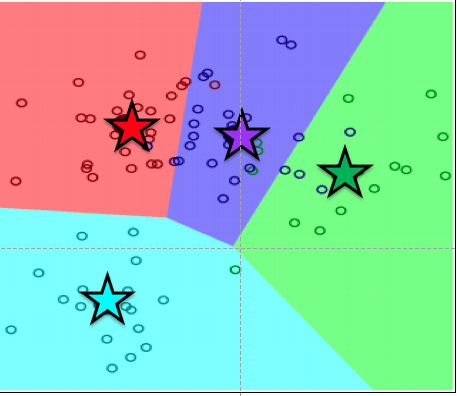
\includegraphics[height=1.24in]{closedset.png}
        }
        {\subfloat[Zooming out to show some open space. \label{fig:zoomed}]{
                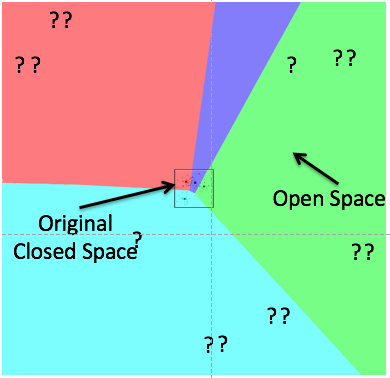
\includegraphics[height=1.24in]{zoomed.png}
                }
        }
       \caption{ The issue of open space can be seen by zooming out from around the training data. 
       Open space is the region far from training samples.  A traditional classifier, e.g., NCM show here,  will label everything including the unknown ``?" inputs. Even points infinitely far away are labeled.}
\end{figure}


By the turn of the century, most A.I. systems stopped explicitly
exploiting the {\em closed world assumptions}, many moving to
probabilistic Bayesian reasoning.
More recently systems have turned to using learning-based models.
Unfortunately, almost all machine learning-based system have
implicitly continued to make that assumption because they classify all inputs into one of their training classes.
Similarly, Bayesian reasoning implicitly retains the closed world
assumption.
Research often seek Closed set classifiers, that approximate the Bayesian
optimal posterior probability, $P(C_l |x';{\cal C}_1, 
\hdots, {\cal C}_M), l \in \{1,\hdots, M\}$, for a fixed set of
classes, where $x'$ is an input sample, $l$ is the index of class
${\cal C}_l$ (a particular known class), and $M$ is the number of
known classes.
When $\Omega$ unknown classes appear at query time, however, the
Bayesian optimal posterior becomes $P(C_{\tilde{l}} |x';{\cal C}_1,
 \hdots, {\cal C}_M, U_{M+1}, \hdots, U_{M+\Omega})$, which cannot be
computed/modeled because classes $U_{M+1}$ through $U_\Omega$ are
unknown.
Even the core law of total probability, essential in Bayes theorem,
cannot be applied unless one presumes the probability of all unknown
inputs is known.
In other words, using Bayes theorem requires implicitly making a
closed world assumption.
For classifiers that assess confidence in terms of signed distance from a decision boundary, or some calibration thereof, this misclassification will occur with high confidence if the unknown is far from any known data --- a result that is very misleading.

Until recently, almost all evaluations of machine-learning-based recognition algorithms have implicitly been  ``closed set" whereby the system is only tested on classes known at training time. A more realistic scenario for applications is accepting that the world is an open set of objects, that our knowledge is always incomplete, and thus that unknown classes should be submitted to an algorithm during testing.  This paper reviews and extends the formalizations of {\bf open set recognition}  \cite{Walter_openset,walter2014} and   \textbf{open world recognition}  \cite{bendale2015towards}, collectively open recognition.

Related, but formally separate from open recognition, are the approaches that use classifiers with rejection  \cite{chow1970optimum,matan1990handwritten,fumera2002support,zhang2006ro,bartlett2008classification,Grandvalet_nips08_reject}, novelty/anomaly/outlier detection  \cite{hodge2004survey,markou2003novelty}.  These can help with rejecting unknown inputs but lack the formal properties of provably bounded open space risk.   This paper briefly reviews these areas, recent results,  and explains the difference between them and open recognition. 

OSR is a growing subfield, one that is critical for robust system, as highlighted in a recent {\em AI Magazine} piece \cite{dietterich2017steps}. In the five years following our formalization of OSR in  \cite{Walter_openset}, the problem has received significant attention. The work in this area has received hundreds of citations from a wide range of application areas that need, or are using, OSR including:
{\small
\begin{itemize}[nosep]
\item Audio analysis \cite{battaglino_open-set_2016,krstulovic_audio_2018},
\item Automatic Target Recognition \cite{scherreik_open_2016,scherreik_multi-class_2016,roos_probabilistic_2017},
\item Autonomous Navigation/Mobile Robitcs  \cite{zamora_novel_2016,sunderhauf_place_2016}, 
\item Biomtrics \cite{chiachia_learning_2014,pinto_using_2015,rattani_open_2015,juefei-xu_multi-class_2016,gunther_toward_2017,perera_extreme_2017,bao2018towards}, 
\item Cyber Intrusion/Malware Detection \cite{henrydoss_incremental_2017,cruz_open_2017,rudd_survey_2017},
\item Data Fusion \cite{neira_data-fusion_2018},
\item Domain Adaption \cite{gopalan_domain_2015,busto_open_2017}, 
\item Forensics \cite{costa_open_2014,rocha_authorship_2017,navarro_connecting_2018},
\item Lifelong Learning  \cite{chen_lifelong_2016,rebuffi_icarl:_2017},
\item Natural Language \cite{prakhya_open-set_2017,doan_overcoming_2017,grave_unbounded_2017}, 
\item Novelty Detection  \cite{bodesheim_local_2015,lazzaretti_novelty_2016,schultheiss_finding_2017},
\item Package Authentication \cite{schraml_feasibility_2017},  
\item Unmanned Aerial Systems and Aerial Imagery \cite{poitevin_challenges_2017,bapst_open_2017},
and
\item Zero-shot learning  \cite{lampert_attribute-based_2014,chao_empirical_2016,xian_zero-shot_2017,fu_recent_2018,xian_zero-shot_2018}
\end{itemize}
}
There have also been papers developing their own models/algorithms for OSR, e.g. 
\cite{cardoso_bounded_2015,liu_modular_2016,ferreira_convolutional_2017,zhang_sparse_2017,mu_classification_2017,gunther2017unconstrained,neal2018open,bansal2018coverage}



When using classic ``explainable" features for a problem, the problem of open recognition can be well formulated in either image or feature space.  With the shift to deep networks, which combines learning features and learning the classifier,  the problem becomes more difficult and is still largely unsolved.  The paper ends with a discussion of some of the issues that make open set deep learning so tricky, and so vital as we move toward intelligent systems.


At the core of intelligence is the ability to recognize when we do not know something, analyze the need to learn about it, and then, when needed, to adapt and learn it -- a process we call open world learning. 
As research moves towards building intelligent systems and deploying machine learning-based systems, this is a critical but understudied area of research. The fundamental research question addressed in this paper is how to formally address the unknown in machine learning systems. This paper reviews formal approaches for handling those issues, but the problem is far from solved.  In our ever-changing world,  we recommend you {\em do not trust a claim of intelligence that does not admit when it does not know or does not continue to learn.}     


\section{Formalizing Open Set Recognition}
\label{sec:theory}



We introduced the first formalization of open recognition in
 \cite{Walter_openset} with essential properties: bounding the open
space risk and ideally balancing it with empirical risk.
Empirical risk, measured on training data, is easy to define and
practical to optimize over, but how to extend the model to capture the risk from
unknown inputs is the critical issue for OSR.
That paper argued the essential element of OSR is minimizing the volume
of space representing the learned recognition function $f$, outside
the reasonable support of the positive samples, because clusters of
unknown samples in initially unlabeled regions are more likely to be
negatives and increase the recognition error.
Note, this is entirely different from the classic binary classifier
approach, which tries to label everything, and often generalization to
infinite space in some directions.
Let's proceed to formalize this idea.
Let $f$ be a measurable recognition function over input space $\cal
X$, for known valid class ${\hat V}$. Let $S_{\hat V}$ be a union
of balls of radius $r_o$ that includes all of the training examples
for all known $x \in {\hat V}$, let ${\cal O}$ be the open space with
$\cal O \subset= X-S_{\hat V}$.
Open space risk $R_{\cal O}(f)$ for class ${\hat V}$ can be defined as $R_{{\cal O}}(f) = \frac{\int_{{\cal O}} f_{\hat V}(x) dx}{\int_{S_{\hat V}} f_{\hat V}(x) dx} $, where open space risk is considered to be the relative measure of positively labeled open space compared to the overall measure of positively labeled space.
Following  \cite{Walter_openset} we can formally define the OSR problem as follows:
\begin{mydef}
\label{def:openset}
\textup{The Open Set Recognition (OSR) Problem:}\\
Using training data with positive
samples $v_i \in{\hat V}$, and other known class samples  $k_j \in {\hat   K}$, and an empirical data error/accuracy measure $\cal E$, find a measurable recognition function $f\in \cal H, $ where $f(x)>0$ implies positive recognition for class ${\hat V}$, and $f$ is defined as minimizing the OSR error:
{\small
\begin{equation}
\label{eq:openspacerecognition}
\argmin_{f \in {\cal H}} \left\{{ R_{{\cal O}}(f)   + \lambda_r  {\cal E}(f(v_{i}); f(k_{j}))}\right\}
\end{equation}
subject to 
\begin{equation}
m\alpha\ \le \sum\limits_{i=1}^m \phi(f(v_{i}))  \quad  \mathrm{ and } \quad   n\beta \ge \sum\limits_{j=1}^n \label{eq:sampleerror}
\phi(f(k_{j}))
\end{equation}
}where $\lambda_r$ specifies the regularization tradeoff between open space risk and
empirical risk, where $\alpha\ge 0$ and $\beta\ge0$ allow a prescribed limit on
true positive and/or false positive rates, and  $\phi(z)$ is a given loss
function, e.g. the  classic soft margins hinge loss $\phi(z)=max(0,1-z)$ or squared hinge loss $\phi(z)=max(0,1-z)^2$ functions.
\end{mydef}



The full regularized optimization for OSR error can be difficult.  However,  since empirical risk is always bounded,  it is straightforward  to see that if $f(x)>0$ for a infinite amount of space, then $R_{{\cal O}}(f)= \infty$ and such an $f$ cannot even be an approximately optimal solution because its open set risk is unbounded while the function $f(x)=0$ always has bounded OSR error.     For that reason we consider a minimal requirement for an algorithm to be called a formal OSR algorithm to be $R_{{\cal O}}(f) < B$ for a finite bound $B$.   Any function that realizes such a finite OSR error will be within some constant of the optimal error. In our various papers on the topic, \cite{walter2014,bendale2015towards,junior2016specialized,rudd2018extreme},  we show multiple different ways to find algorithms with bounded open space error.  

\section{Extensions: CAP and Open World Recognition}
\begin{figure}
\center
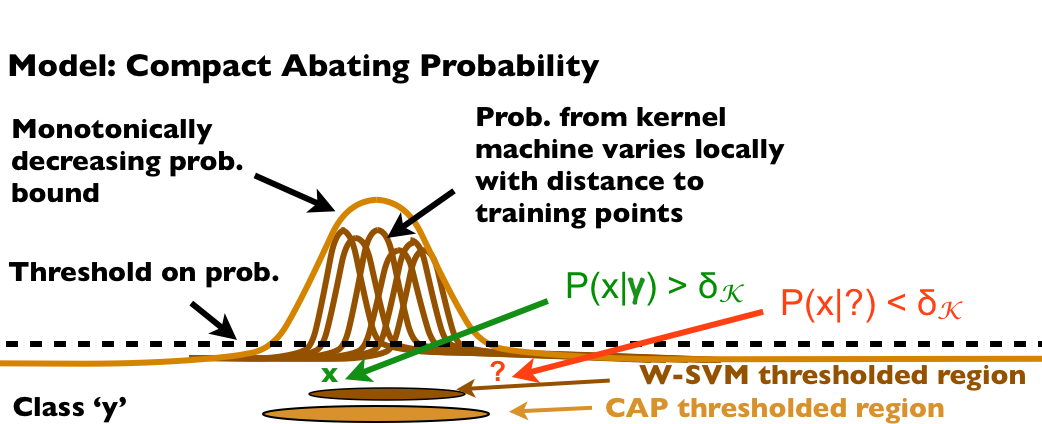
\includegraphics[width=.8\columnwidth]{CAP.png}
\caption{Compact Abating Probability model which when, thresholded, can bound open space risk. CAP models are often used in novelty/anomaly/outlier detectors.}
\label{fig:cap}
\end{figure}


In  \cite{walter2014}, we introduced the idea of a \textit{Compact Abating Probability} or CAP model, and showed that such models always have a bounded OSR error.
The basic idea of a CAP model, see Fig.~\ref{fig:cap}, is that if the region of support for the classifier is decreasing in all directions away from the training samples, then thresholding it will bound the open space risk.  
With the theorems in that paper, we showed that some models already in the literature, such as a thresholded RBF one-class SVM, formally bound open-space risk.
The paper also introduces the WSVM, which was far more accurate than any prior OSR algorithm.  The WSVM uses Extreme Value Theory (EVT) to calibrate and combine multiple kernel-SVMs with a CAP model.    



In an attempt to reduce the computational cost compared to the WSVM, we developed another variant, the Pi-SVM,  \cite{Lalit-eccv}.
While it was generally as accurate and sometimes more accurate than the WSVM, at a small fraction of the cost, we could not prove that the algorithm always had bounded open space risk.
Examining why, we recognized that the same issue occurred for a regular SVM, and proved that an RBF-SVM with a CAP consistent kernel would have bounded open space risk {\em if and only if}, all of the bias terms are negative.
The negative bias property might also be why some SVM-based systems do not have a problem with unknown inputs -- if the data happens to result in kernels with negative bias terms, then the SVMs will have bounded open space risk for that data. We developed an SVM variant, the specialized SVM  \cite{junior2016specialized}, which ensures negative bias and hence OSR. 
While any decreasing function can be a CAP model, and many existing novelty/anomaly/outlier detectors use them,  the modeling of the tails of the distribution, the extreme values, is very critical to balancing open set risk and classification accuracy.  That is why most our work turned to EVT.


In the follow-on work of  \cite{bendale2015towards} we formally defined
and extended the OSR problem to \textit{open world recognition}.  An
effective open-world recognition system must efficiently perform four
tasks: detect unknowns, choose which points to label for addition
to the model, label the points, and update the model.  While
something like the WSVM could formally be used for incremental
learning, since there are incremental SVM tools,
 \cite{caragea2000incremental}, those
algorithms do not scale well.   A simple and more efficient algorithm,
nearest non-outlier (NNO), was proposed as part our open
world recognition approach.   The proofs of  \cite{walter2014} were extended to handle transformations of CAP models, e.g., combinations of multiple cap models also bound open space risk, and thus NNO offered a formal solution to open world recognition.   Those proofs also allowed us to show that thresholding many widely used density-based models such as  GMMs or KDE, are also provably OSR algorithms. 
Unfortunately, NNO was not very accurate, as the algorithm used thresholded distances from the nearest class mean as its decision function and otherwise ignored distributional information.    Weak classifiers are a persistent problem for incremental learning: it is not immediately obvious how one might extend class boundary models from classical machine learning theory,  \textit{e.g.},  kernel machines, to incorporate both incremental learning and open set constraints. 

In \cite{rudd2018extreme}, we developed the Extreme Value Machine (EVM), a new non-linear radial basis function approach that supports both high-quality non-linear decision boundaries and efficient incremental learning. We proved that the EVM has bounded open space risk, and significantly more accurate than NNO on large-scale Image-Net testing using deep features. 



\section{Approaches that sometimes solve OSR}
%Rejection, Background, Novelty, and Anamonly Detection

In this section, we discuss approaches some people argue address OSR and explain why these algorithms generally have an infinite open set risk. 

A common question is why a pure detection system with a binary output, e.g., a face detector, is not a solution, and why it does not already limit its open set risk.
It turns out that for some detection systems, in particular, those
that use GMMs, kernel density estimators, RBF SVMs or Support Data
Descriptors (SDD), they do because have bounded open space risk.
However, any detector that uses linear classifiers, HAAR cascades, or
Softmax-based classifiers, will almost always have an unbounded open set risk, and hence
does not solve OSR.



``What about classifier with rejection?"
you might ask.
``Doesn't that solve the OSR problem?"
The problem of rejecting some inputs in learning is more than 60 years old, see \cite{chow1957optimum}.
Since its earliest days,  the focus of rejecting has been the ambiguity between classes, not for addressing unknown inputs.
As \cite{chow1970optimum} put it ``The option to reject is introduced to safeguard against excessive misrecognition; it converts potential misrecognition into rejection."
Chow's papers derive optimal thresholds for that multi-class recognition, assuming probabilities of classes are given over the whole feature space.
The paper's thresholds were for optimizing the ambiguous regions between classes -- it has the infinite regions of acceptance and infinite regions of rejection.
Uncertainty is high near the decision boundary most classifiers increase confidence with distance from the decision boundary.  Thus an unknown far from the boundary is not only incorrectly labeled but will be incorrectly classified with very high confidence.
Even the majority of recent classifiers with reject-options \cite{fumera2002support,zhang2006ro,Grandvalet_nips08_reject,bartlett2008classification,wegkamp-11}, all have the same issues and formally don't solve OSR problems because they can and generally have infinite positively labeled open space, hence infinite open space risk.
The only classification with rejection options that do solve OSR are those that also satisfy the CAP criterion discussed above, e.g., a K-nearest neighbor with a threshold on an appropriate measure \cite{li2005open} or threshold on one or more one-class classifiers \cite{tax2008growing,liu_modular_2016}, in which cases there exists a threshold that will produce finite open space risk.

Novelty and  anomaly detection algorithms \cite{bodesheim_local_2015,lazzaretti_novelty_2016,schultheiss_finding_2017,bansal2018coverage} are solving different but related problems.  Most such techniques apply a distributional model that is thresholded to detect the anomaly. They bound open space risk;  they inspired our CAP model.   However, their formulations do not balance open space risk with multi-class recognition risk as in Eq~\ref{eq:openspacerecognition}.   They are only OSR for one-class problems.   We can summarize the relationship informally as:\\ \centerline{\bf OSR $\approx$  Novelty-detection + multi-class recognition.}



\section{Open Set  Deep Networks}

The problem of open recognition is well formulated in either image or feature space, but people normally think of the world in image space.  The above formal work on OSR was all done in ``explainable” feature spaces, i.e., there existed a well-behaved mapping between input and the feature spaces.   
Due to the large complexity and the black box nature of deep networks, more than often this mapping does not exist.
Moreover, their increased applications in the real world open them to a vast majority of unknown inputs, hence addressing OSR for deep networks is essential.
We follow the OSR definition and just deal with the problem of OSR in testing, leaving for future work that this ignores the potential problem of unknowns showing up in the training data. 


While rejecting unknown inputs by thresholding the network score is common, e.g., \cite{matan1990handwritten,de2000reject},  thresholding softmax is problematic.
Almost since its inception  \cite{bridle1989probablistic}, softmax has been known to bias the probabilities towards a particular class even though the difference between the logit values of the winning class and other classes is minimal.
This was highlighted by  \cite{matan1990handwritten} who note that softmax would increase scores for a particular class even though they may have very limited activation on the logit level.
In order to train the network to provide better logit values, they include an additional parameter $\alpha$ in the softmax loss by modifying the loss function as:
$S_c=\log e^{l_c}/\left({e^\alpha}+\sum_{c'=1}^{C}e^{l_{c'}}\right)$.
During training, this forces a higher loss when the logit values, $l$, are smaller than $\alpha$ , and decrease the softmax scores when all logit values were smaller than $\alpha$.
This additional parameter can be interpreted as an additional node in the output layer that is not updated during back-propagation.
Note, however, that like the other rejection approaches, this carves out a small region around the origin, and potentially between two classes as ``none of the above," and still leaves infinite open space risk and hence does not solve OSR.   
In addition, there is also active research in network \emph{uncertainty estimation} and  \cite{gal2016dropout,lakshminarayanan2017simple,mor2018confidence}, which the authors of such papers say can be thresholded to reject outliers. While more advanced than  \cite{matan1990handwritten}, these still suffer from infinite open space risk and hence do not solve OSR.




Another decades-old rejection approach used in neural networks is to add an  ``garbage” class  \cite{linden1989inversion} or ``background” class  \cite{chang1994figure}.
The ``background’' class is more effective than just thresholding uncertainty and hence is part of almost all modern multi-class detector such as   \cite{liu2016ssd,girshick2015fast,ren2015faster,zhang2018pedestrian}.
It must be noted that this background classifier just adds another class to reject instances not belonging to any of the known classes, but leaves infinite open space beyond each of the known classes.  For different Bayesian Neural Networks  \cite{ghosh2016assumed}, like any Bayes-based approach,  makes a closed world assumption for all probability computations and is not suitable for OSR. 

Background-class based approaches capture some of the ``known unknowns.” However, background approaches  do not limit the space to have finite positively labeled open space, and hence  they are formally not OSR.
Background class modeling can work pretty well for self-consistent  datasets like PASCAL  \cite{everingham2010pascal} and  MS-COCO  \cite{lin2014microsoft}, where  algorithms are often evaluated. However,  the non-OSR property is a likely a source of ``negative” dataset bias  \cite{tommasi2017deeper} and limits application in the real world where the negative space has near infinite variety of inputs that should be rejected.





The OpenMax approach in  \cite{bendale2016openmax} is the first deep network approach to solve OSR formally.
OpenMax uses EVT to define a per-class CAP model around the deep features of each class and then thresholds that probability to reject unknown inputs.
The paper uses the penultimate layer, the logits, as a high-dimensional
deep feature vector. However, the OpenMax approach could be used with any deep feature layer.
Using the EVT model built from the positive instances training samples, it builds a per-class EVT probabilistic model of the input not belonging to that class, combining these in the OpenMax estimate of each class probability including the probability of it being unknown.
Though this approach provides the first steps to formally address the
open set issue for deep networks, it is an offline solution after the
network had already been trained.  Our more recent EVM model,
 \cite{rudd2018extreme},  also provides a non-linear radial basis
function approach based on EVT, but it provides a more flexible and
more powerful representation model for OpenMax than the single class
mean used in the original OpenMax paper. Neither of these models,
however, are used in training the deep features. 


One can see that a few networks with distance-based loss functions, such as center loss  \cite{wen2016discriminative} and its variants, can be converted into an OSR network by simple thresholding on Euclidean distance from each class center as well as by applying an OpenMax layer. 


More recent work on deep network  \cite{Dhamija_NIPS18} seeks to train networks that handle unknowns by combining softmax with a new loss function which forces known unknown samples, i.e., background classes, to have a small feature magnitude.
While empirically the approach is considerably better than either using a background class or OpenMax, it formally has an unbounded open space risk.

The final OSR issue related to deep networks is related to the question of what one means by being far from training data.  For traditional features, it was generally fine to think about it in either input space or feature space.  However, for deep networks,  adversarial examples \cite{szegedy2013intriguing} and fooling images  \cite{nguyen2015deep}  clearly break that parallelism.  Both of these approaches produce images that are close in one space and far in the other.  Moreover, while OpenMax was able to detect and mitigate most of the fooling images and simple adversarial examples, using an attack that goes after deep features rather than the end-to-end network we can manipulate just about any image so that it matches the features of a target and were easily able to defeat OpenMax \cite{rozsa2017adversarial}.  As of this writing, we are unaware of any defense against this attack.  Thus, for deep networks, while we can develop OSR in feature space, it is not clear how to make them robust in image space, which is, of course, where the real world projects. 



\section{Conclusion}

While machine learning and deep networks are providing great advances, and many applications areas are awash with data, no amount of training will prepare the system for all unknown inputs.    
Rejecting uncertain inputs is not enough  --- uncertain is not unknown, and unknowns are often labeled with confidence.   Novelty/anomaly/outlier detection alone is not sufficient because the proper handling of unknowns involves balancing the risk of the unknown with the risks from recognition errors.  With almost all deep networks, unknowns map into the same space as knowns and are not easily rejected as outliers.


While significant progress has been made, as the astute reader who was checking references while reading may have noted, more than a dozen of the references have titles like ``Towards..."; this is an emerging area with more unknowns than knowns.
Open set problems are often challenging because they must balance maintaining accuracy on the core problem with handling the unknown unknowns.
However, dealing with the unknown is essential, and we need systems explicitly designed to handle the unknown.
{\bf {Do not fear the unknown ---} {join us in taming it.}
}




\begin{quote}
\em
``For any scientist, the real challenge is not to stay within the secure garden of the known but to venture out into the wilds of the unknown.” --
  \cite{du2017great}    
\end{quote}






\fontsize{9.5pt}{10.0pt} \selectfont
\fontsize{9.1pt}{10pt}\selectfont
%\fontsize{9pt}{10pt}\selectfont %smallest allowed

%References and End of Paper
%These lines must be placed at the end of your paper
%\bibliography{aaai18}
%\bibliographystyle{aaai}

\begin{thebibliography}{}

\bibitem[\protect\citeauthoryear{Bansal and Weld}{2018}]{bansal2018coverage}
Bansal, G., and Weld, D.~S.
\newblock 2018.
\newblock A coverage-based utility model for identifying unknown unknowns.
\newblock In {\em Proc. of AAAI}.

\bibitem[\protect\citeauthoryear{Bao \bgroup et al\mbox.\egroup
  }{2018}]{bao2018towards}
Bao, J.; Chen, D.; Wen, F.; Li, H.; and Hua, G.
\newblock 2018.
\newblock Towards open-set identity preserving face synthesis.
\newblock In {\em IEEE CVPR}.

\bibitem[\protect\citeauthoryear{Bapst \bgroup et al\mbox.\egroup
  }{2017}]{bapst_open_2017}
Bapst, A.~B.; Tran, J.; Koch, M.~W.; Moya, M.~M.; and Swahn, R.
\newblock 2017.
\newblock Open set recognition of aircraft in aerial imagery using synthetic
  template models.
\newblock In {\em Automatic {Target} {Recognition} {XXVII}}, volume 10202,
  1020206.

\bibitem[\protect\citeauthoryear{Bartlett and
  Wegkamp}{2008}]{bartlett2008classification}
Bartlett, P., and Wegkamp, M.
\newblock 2008.
\newblock Classification with a reject option using a hinge loss.
\newblock {\em In JMLR} 9:1823--1840.

\bibitem[\protect\citeauthoryear{Battaglino, Lepauloux, and
  Evans}{2016}]{battaglino_open-set_2016}
Battaglino, D.; Lepauloux, L.; and Evans, N.
\newblock 2016.
\newblock The open-set problem in acoustic scene classification.
\newblock In {\em 2016 {IEEE} {Int.} {Workshop} on {Acoustic} {Signal}
  {Enhancement} ({IWAENC})},  1--5.
\newblock IEEE.

\bibitem[\protect\citeauthoryear{Bendale and Boult}{2015}]{bendale2015towards}
Bendale, A., and Boult, T.
\newblock 2015.
\newblock Towards open world recognition.
\newblock In {\em IEEE CVPR},  1893--1902.

\bibitem[\protect\citeauthoryear{Bendale and Boult}{2016}]{bendale2016openmax}
Bendale, A., and Boult, T.~E.
\newblock 2016.
\newblock Towards open set deep networks.
\newblock In {\em IEEE CVPR},  1563--1572.

\bibitem[\protect\citeauthoryear{Bodesheim \bgroup et al\mbox.\egroup
  }{2015}]{bodesheim_local_2015}
Bodesheim, P.; Freytag, A.; Rodner, E.; and Denzler, J.
\newblock 2015.
\newblock Local novelty detection in multi-class recognition problems.
\newblock In {\em IEEE WACV},  813--820.

\bibitem[\protect\citeauthoryear{Bridle}{1989}]{bridle1989probablistic}
Bridle, J.
\newblock 1989.
\newblock Probablistic interpretation of feedforward classification network
  outputs, with relationships to statistical pattern recognition.
\newblock {\em Neuro-computing: Algorithms, Architectures}.

\bibitem[\protect\citeauthoryear{Busto and Gall}{2017}]{busto_open_2017}
Busto, P.~P., and Gall, J.
\newblock 2017.
\newblock Open {Set} {Domain} {Adaptation}.
\newblock In {\em {ICCV}},  754--763.

\bibitem[\protect\citeauthoryear{Caragea, Silvescu, and
  Honavar}{2000}]{caragea2000incremental}
Caragea, D.; Silvescu, A.; and Honavar, V.
\newblock 2000.
\newblock Incremental and distributed learning with support vector machines.
\newblock In {\em AAAI},  1067.

\bibitem[\protect\citeauthoryear{Cardoso, França, and
  Gama}{2015}]{cardoso_bounded_2015}
Cardoso, D.~O.; França, F.; and Gama, J.
\newblock 2015.
\newblock A bounded neural network for open set recognition.
\newblock In {\em Neural {Networks} ({IJCNN}), 2015 {Int.} {Joint} {Conf.} on},
   1--7.
\newblock IEEE.

\bibitem[\protect\citeauthoryear{Chang and Lippmann}{1994}]{chang1994figure}
Chang, E.~I., and Lippmann, R.~P.
\newblock 1994.
\newblock Figure of merit training for detection and spotting.
\newblock In {\em NIPS},  1019--1026.

\bibitem[\protect\citeauthoryear{Chao \bgroup et al\mbox.\egroup
  }{2016}]{chao_empirical_2016}
Chao, W.-L.; Changpinyo, S.; Gong, B.; and Sha, F.
\newblock 2016.
\newblock An empirical study and analysis of generalized zero-shot learning for
  object recognition in the wild.
\newblock In {\em ECCV},  52--68.
\newblock Springer.

\bibitem[\protect\citeauthoryear{Chen and Liu}{2016}]{chen_lifelong_2016}
Chen, Z., and Liu, B.
\newblock 2016.
\newblock Lifelong machine learning.
\newblock {\em Synthesis Lect. on Art. Int. and Machine Learning} 10(3):1--145.

\bibitem[\protect\citeauthoryear{Chiachia \bgroup et al\mbox.\egroup
  }{2014}]{chiachia_learning_2014}
Chiachia, G.; Falcao, A.~X.; Pinto, N.; Rocha, A.; and Cox, D.
\newblock 2014.
\newblock Learning person-specific representations from faces in the wild.
\newblock {\em IEEE TIFS} 9(12):2089--2099.

\bibitem[\protect\citeauthoryear{Chow}{1957}]{chow1957optimum}
Chow, C.-K.
\newblock 1957.
\newblock An optimum character recognition system using decision functions.
\newblock {\em IRE Trans. on Ele. Comp.} 4:247--254.

\bibitem[\protect\citeauthoryear{Chow}{1970}]{chow1970optimum}
Chow, C.
\newblock 1970.
\newblock On optimum recognition error and reject tradeoff.
\newblock {\em IEEE Trans. Info. Theory} 16(1):41--46.

\bibitem[\protect\citeauthoryear{Costa \bgroup et al\mbox.\egroup
  }{2014}]{costa_open_2014}
Costa, F. d.~O.; Silva, E.; Eckmann, M.; Scheirer, W.~J.; and Rocha, A.
\newblock 2014.
\newblock Open set source camera attribution and device linking.
\newblock {\em Pat. Rec. Letters} 39:92--101.

\bibitem[\protect\citeauthoryear{Cruz \bgroup et al\mbox.\egroup
  }{2017}]{cruz_open_2017}
Cruz, S.; Coleman, C.; Rudd, E.~M.; and Boult, T.~E.
\newblock 2017.
\newblock Open set intrusion recognition for fine-grained attack
  categorization.
\newblock In {\em {IEEE} Tech. for {Homeland} {Security}}.

\bibitem[\protect\citeauthoryear{De~Stefano, Sansone, and
  Vento}{2000}]{de2000reject}
De~Stefano, C.; Sansone, C.; and Vento, M.
\newblock 2000.
\newblock To reject or not to reject: that is the question-an answer in case of
  neural classifiers.
\newblock {\em IEEE TSMC, Part C} 30(1):84--94.

\bibitem[\protect\citeauthoryear{Dhamija, G\"unther, and
  Boult}{2018}]{Dhamija_NIPS18}
Dhamija, A.; G\"unther, M.; and Boult, T.~E.
\newblock 2018.
\newblock Reducing network agnostophobia.
\newblock In {\em NIPS}.

\bibitem[\protect\citeauthoryear{Dietterich}{2017}]{dietterich2017steps}
Dietterich, T.~G.
\newblock 2017.
\newblock Steps toward robust artificial intelligence.
\newblock {\em AI Magazine} 38(3):3--24.

\bibitem[\protect\citeauthoryear{Doan and Kalita}{2017}]{doan_overcoming_2017}
Doan, T., and Kalita, J.
\newblock 2017.
\newblock Overcoming the challenge for text classification in the open world.
\newblock In {\em Computing and {Communication} {Workshop} and {Conf.}}
\newblock IEEE.

\bibitem[\protect\citeauthoryear{Du~Sautoy}{2017}]{du2017great}
Du~Sautoy, M.
\newblock 2017.
\newblock {\em The Great Unknown: Seven Journeys to the Frontiers of Science}.
\newblock Penguin.

\bibitem[\protect\citeauthoryear{Everingham \bgroup et al\mbox.\egroup
  }{2010}]{everingham2010pascal}
Everingham, M.; Van~Gool, L.; Williams, C.~K.; Winn, J.; and Zisserman, A.
\newblock 2010.
\newblock The pascal visual object classes (voc) challenge.
\newblock {\em Int. {J}ournal of {C}omputer {V}ision} 88(2):303--338.

\bibitem[\protect\citeauthoryear{Ferreira and
  Giraldi}{2017}]{ferreira_convolutional_2017}
Ferreira, A., and Giraldi, G.
\newblock 2017.
\newblock Convolutional {Neural} {Network} approaches to granite tiles
  classification.
\newblock {\em Expert Systems with Applications} 84:1--11.

\bibitem[\protect\citeauthoryear{Fu \bgroup et al\mbox.\egroup
  }{2018}]{fu_recent_2018}
Fu, Y.; Xiang, T.; Jiang, Y.-G.; Xue, X.; Sigal, L.; and Gong, S.
\newblock 2018.
\newblock Recent advances in zero-shot recognition: {Toward} data-efficient
  understanding of visual content.
\newblock {\em IEEE Signal Processing Magazine} 35(1):112--125.


\bibitem[\protect\citeauthoryear{Fumera and Roli}{2002}]{fumera2002support}
Fumera, G., and Roli, F.
\newblock 2002.
\newblock Support vector machines with embedded reject option.
\newblock In {\em Pat. Rec. with Support Vector Machines}. Springer.
\newblock  68--82.

\bibitem[\protect\citeauthoryear{Gal and Ghahramani}{2016}]{gal2016dropout}
Gal, Y., and Ghahramani, Z.
\newblock 2016.
\newblock Dropout as a bayesian approximation: Representing model uncertainty
  in deep learning.
\newblock In {\em Int. Conf. on Machine Learning},  1050--1059.

\bibitem[\protect\citeauthoryear{Ghosh, Delle~Fave, and
  Yedidia}{2016}]{ghosh2016assumed}
Ghosh, S.; Delle~Fave, F.~M.; and Yedidia, J.~S.
\newblock 2016.
\newblock Assumed density filtering methods for learning bayesian neural
  networks.
\newblock In {\em AAAI},  1589--1595.

\bibitem[\protect\citeauthoryear{Girshick}{2015}]{girshick2015fast}
Girshick, R.
\newblock 2015.
\newblock Fast {R-CNN}.
\newblock In {\em IEEE ICCV},  1440--1448.

\bibitem[\protect\citeauthoryear{Gopalan \bgroup et al\mbox.\egroup
  }{2015}]{gopalan_domain_2015}
Gopalan, R.; Li, R.; Patel, V.~M.; and Chellappa, R.
\newblock 2015.
\newblock Domain adaptation for visual recognition.
\newblock {\em Foundations and Trends® in Computer Graphics and Vision}
  8(4):285--378.

\bibitem[\protect\citeauthoryear{Grandvalet \bgroup et al\mbox.\egroup
  }{2008}]{Grandvalet_nips08_reject}
Grandvalet, Y.; Rakotomamonjy, A.; Keshet, J.; and Canu, S.
\newblock 2008.
\newblock Support vector machines with a reject option.
\newblock In {\em NIPS},  537--544.
\newblock Curran Associates, Inc.

\bibitem[\protect\citeauthoryear{Grave, Cisse, and
  Joulin}{2017}]{grave_unbounded_2017}
Grave, E.; Cisse, M.~M.; and Joulin, A.
\newblock 2017.
\newblock Unbounded cache model for online language modeling with open
  vocabulary.
\newblock In {\em NIPS},  6042--6052.

\bibitem[\protect\citeauthoryear{G{\"u}nther \bgroup et al\mbox.\egroup
  }{2017}]{gunther2017unconstrained}
G{\"u}nther, M.; Hu, P.; Herrmann, C.; Chan, C.~H.; Jiang, M.; Yang, S.;
  Dhamija, A.~R.; Ramanan, D.; Beyerer, J.; Kittler, J.; et~al.
\newblock 2017.
\newblock Unconstrained face detection and open-set face recognition challenge.
\newblock In {\em IEEE Int. Joint. Conf. Biometrics},  697--706.

\bibitem[\protect\citeauthoryear{Günther \bgroup et al\mbox.\egroup
  }{2017}]{gunther_toward_2017}
Günther, M.; Cruz, S.; Rudd, E.~M.; and Boult, T.~E.
\newblock 2017.
\newblock Toward open-set face recognition.
\newblock In {\em IEEE CVPR Workshops}.

\bibitem[\protect\citeauthoryear{Henrydoss \bgroup et al\mbox.\egroup
  }{2017}]{henrydoss_incremental_2017}
Henrydoss, J.; Cruz, S.; Rudd, E.~M.; and Boult, T.~E.
\newblock 2017.
\newblock Incremental {Open} {Set} {Intrusion} {Recognition} {Using} {Extreme}
  {Value} {Machine}.
\newblock In {\em Machine {Learning} and {Applications} ({ICMLA}), 2017 16th
  {IEEE} {Int.} {Conf.} on},  1089--1093.
\newblock IEEE.

\bibitem[\protect\citeauthoryear{Hewitt and Jong}{1983}]{hewitt83analyzing}
Hewitt, C., and Jong, P.~D.
\newblock 1983.
\newblock Analyzing the roles of descriptions and actions in open system.
\newblock In {\em Proceedings of AAAI-83},  162--167.
\newblock See also AI Lab Memo727,
  \url{http://www.dtic.mil/dtic/tr/fulltext/u2/a133614.pdf}.

\bibitem[\protect\citeauthoryear{Hodge and Austin}{2004}]{hodge2004survey}
Hodge, V.~J., and Austin, J.
\newblock 2004.
\newblock A survey of outlier detection methodologies.
\newblock {\em Artificial Intelligence Review} 22(2):85--126.

\bibitem[\protect\citeauthoryear{Jain, Scheirer, and Boult}{2014}]{Lalit-eccv}
Jain, L.~P.; Scheirer, W.~J.; and Boult, T.~E.
\newblock 2014.
\newblock Multi-class open set recognition using probability of inclusion.
\newblock In {\em ECCV}.

\bibitem[\protect\citeauthoryear{Juefei-Xu and
  Savvides}{2016}]{juefei-xu_multi-class_2016}
Juefei-Xu, F., and Savvides, M.
\newblock 2016.
\newblock Multi-class {Fukunaga} {Koontz} discriminant analysis for enhanced
  face recognition.
\newblock {\em Pat. Rec.} 52:186--205.

\bibitem[\protect\citeauthoryear{J{\'u}nior \bgroup et al\mbox.\egroup
  }{2016}]{junior2016specialized}
J{\'u}nior, P. R.~M.; Boult, T.~E.; Wainer, J.; and Rocha, A.
\newblock 2016.
\newblock Specialized support vector machines for open-set recognition.
\newblock {\em arXiv:1606.03802}.

\bibitem[\protect\citeauthoryear{Krstulović}{2018}]{krstulovic_audio_2018}
Krstulović, S.
\newblock 2018.
\newblock Audio event recognition in the smart home.
\newblock In {\em Computational {Analysis} of {Sound} {Scenes} and {Events}}.
  Springer.
\newblock  335--371.

\bibitem[\protect\citeauthoryear{Lakshminarayanan, Pritzel, and
  Blundell}{2017}]{lakshminarayanan2017simple}
Lakshminarayanan, B.; Pritzel, A.; and Blundell, C.
\newblock 2017.
\newblock Simple and scalable predictive uncertainty estimation using deep
  ensembles.
\newblock In {\em NIPS},  6405--6416.

\bibitem[\protect\citeauthoryear{Lampert, Nickisch, and
  Harmeling}{2014}]{lampert_attribute-based_2014}
Lampert, C.~H.; Nickisch, H.; and Harmeling, S.
\newblock 2014.
\newblock Attribute-based classification for zero-shot visual object
  categorization.
\newblock {\em IEEE Trans. on Pattern Analysis and Machine Intelligence}
  36(3):453--465.

\bibitem[\protect\citeauthoryear{Lazzaretti \bgroup et al\mbox.\egroup
  }{2016}]{lazzaretti_novelty_2016}
Lazzaretti, A.~E.; Tax, D. M.~J.; Neto, H.~V.; and Ferreira, V.~H.
\newblock 2016.
\newblock Novelty detection and multi-class classification in power
  distribution voltage waveforms.
\newblock {\em Expert Systems with Applications} 45:322--330.

\bibitem[\protect\citeauthoryear{Li and Wechsler}{2005}]{li2005open}
Li, F., and Wechsler, H.
\newblock 2005.
\newblock Open set face recognition using transduction.
\newblock {\em IEEE transactions on pattern analysis and machine intelligence}
  27(11):1686--1697.

\bibitem[\protect\citeauthoryear{Lin \bgroup et al\mbox.\egroup
  }{2014}]{lin2014microsoft}
Lin, T.-Y.; Maire, M.; Belongie, S.; Hays, J.; Perona, P.; Ramanan, D.;
  Doll{\'a}r, P.; and Zitnick, C.~L.
\newblock 2014.
\newblock Microsoft coco: Common objects in context.
\newblock In {\em ECCV},  740--755.
\newblock Springer.

\bibitem[\protect\citeauthoryear{Linden and
  Kindermann}{1989}]{linden1989inversion}
Linden, A., and Kindermann, J.
\newblock 1989.
\newblock Inversion of multilayer nets.
\newblock In {\em Proc. Int. Joint Conf. Neural Networks}, volume~2,  425--430.

\bibitem[\protect\citeauthoryear{Liu \bgroup et al\mbox.\egroup
  }{2016a}]{liu_modular_2016}
Liu, J.; Miao, Q.; Sun, Y.; Song, J.; and Quan, Y.
\newblock 2016a.
\newblock Modular ensembles for one-class classification based on density
  analysis.
\newblock {\em Neurocomputing} 171:262--276.

\bibitem[\protect\citeauthoryear{Liu \bgroup et al\mbox.\egroup
  }{2016b}]{liu2016ssd}
Liu, W.; Anguelov, D.; Erhan, D.; Szegedy, C.; Reed, S.; Fu, C.-Y.; and Berg,
  A.~C.
\newblock 2016b.
\newblock {SSD}: Single shot multibox detector.
\newblock In {\em ECCV},  21--37.
\newblock Springer.

\bibitem[\protect\citeauthoryear{Markou and Singh}{2003}]{markou2003novelty}
Markou, M., and Singh, S.
\newblock 2003.
\newblock Novelty detection: a review—part 1: statistical approaches.
\newblock {\em Signal Processing} 83(12):2481--2497.

\bibitem[\protect\citeauthoryear{Matan \bgroup et al\mbox.\egroup
  }{1990}]{matan1990handwritten}
Matan, O.; Kiang, R.; Stenard, C.; Boser, B.; Denker, J.; Henderson, D.;
  Howard, R.; Hubbard, W.; Jackel, L.; and Le~Cun, Y.
\newblock 1990.
\newblock Handwritten character recognition using neural network architectures.
\newblock In {\em 4th USPS Adv. Technology Conf.},  1003--1011.

\bibitem[\protect\citeauthoryear{Mensink \bgroup et al\mbox.\egroup
  }{2012}]{mensink2012metric}
Mensink, T.; Verbeek, J.; Perronnin, F.; and Csurka, G.
\newblock 2012.
\newblock Metric learning for large scale image classification: Generalizing to
  new classes at near-zero cost.
\newblock In {\em ECCV}. Springer.

\bibitem[\protect\citeauthoryear{Mor and Wolf}{2018}]{mor2018confidence}
Mor, N., and Wolf, L.
\newblock 2018.
\newblock Confidence prediction for lexicon-free {OCR}.
\newblock In {\em IEEE WACV}.

\bibitem[\protect\citeauthoryear{Mu, Ting, and
  Zhou}{2017}]{mu_classification_2017}
Mu, X.; Ting, K.~M.; and Zhou, Z.-H.
\newblock 2017.
\newblock Classification under streaming emerging new classes: {A} solution
  using completely-random trees.
\newblock {\em IEEE Trans. on Knowledge and Data Engineering} 29(8):1605--1618.

\bibitem[\protect\citeauthoryear{Navarro \bgroup et al\mbox.\egroup
  }{2018}]{navarro_connecting_2018}
Navarro, L.~C.; Navarro, A.~K.; Rocha, A.; and Dahab, R.
\newblock 2018.
\newblock Connecting the dots: {Toward} accountable machine-learning printer
  attribution methods.
\newblock {\em Journal of Visual Communication and Image Representation}
  53:257--272.

\bibitem[\protect\citeauthoryear{Neal \bgroup et al\mbox.\egroup
  }{2018}]{neal2018open}
Neal, L.; Olson, M.; Fern, X.; Wong, W.-K.; and Li, F.
\newblock 2018.
\newblock Open set learning with counterfactual images.
\newblock In {\em ECCV},  613--628.

\bibitem[\protect\citeauthoryear{Neira \bgroup et al\mbox.\egroup
  }{2018}]{neira_data-fusion_2018}
Neira, M. A.~C.; Júnior, P. R.~M.; Rocha, A.; and Torres, R. D.~S.
\newblock 2018.
\newblock Data-{Fusion} {Techniques} for {Open}-{Set} {Recognition} {Problems}.
\newblock {\em IEEE Access} 6:21242--21265.

\bibitem[\protect\citeauthoryear{Nguyen, Yosinski, and
  Clune}{2015}]{nguyen2015deep}
Nguyen, A.; Yosinski, J.; and Clune, J.
\newblock 2015.
\newblock Deep neural networks are easily fooled: High confidence predictions
  for unrecognizable images.
\newblock In {\em IEEE CVPR}.

\bibitem[\protect\citeauthoryear{Perera and Patel}{2017}]{perera_extreme_2017}
Perera, P., and Patel, V.~M.
\newblock 2017.
\newblock Extreme value analysis for mobile active user authentication.
\newblock In {\em 2017 12th {IEEE} {Int.} {Conf.} on {Automatic} {Face} \&
  {Gesture} {Recognition} ({FG} 2017)},  346--353.
\newblock IEEE.

\bibitem[\protect\citeauthoryear{Pinto \bgroup et al\mbox.\egroup
  }{2015}]{pinto_using_2015}
Pinto, A.; Schwartz, W.~R.; Pedrini, H.; and de~Rezende~Rocha, A.
\newblock 2015.
\newblock Using visual rhythms for detecting video-based facial spoof attacks.
\newblock {\em IEEE Trans. on Information Forensics and Security}
  10(5):1025--1038.

\bibitem[\protect\citeauthoryear{Poitevin, Pelletier, and
  Lamontagne}{2017}]{poitevin_challenges_2017}
Poitevin, P.; Pelletier, M.; and Lamontagne, P.
\newblock 2017.
\newblock Challenges in detecting {UAS} with radar.
\newblock In {\em Security {Technology} ({ICCST}), 2017 {Int.} {Carnahan}
  {Conf.} on}.
\newblock IEEE.

\bibitem[\protect\citeauthoryear{Prakhya, Venkataram, and
  Kalita}{2017}]{prakhya_open-set_2017}
Prakhya, S.; Venkataram, V.; and Kalita, J.
\newblock 2017.
\newblock Open-{Set} {Deep} {Learning} for {Text} {Classification}.
\newblock {\em Machine Learning in Computer Vision and NLP}.

\bibitem[\protect\citeauthoryear{Rattani, Scheirer, and
  Ross}{2015}]{rattani_open_2015}
Rattani, A.; Scheirer, W.~J.; and Ross, A.
\newblock 2015.
\newblock Open set fingerprint spoof detection across novel fabrication
  materials.
\newblock {\em IEEE Trans. on Information Forensics and Security}
  10(11):2447--2460.

\bibitem[\protect\citeauthoryear{Rebuffi \bgroup et al\mbox.\egroup
  }{2017}]{rebuffi_icarl:_2017}
Rebuffi, S.-A.; Kolesnikov, A.; Sperl, G.; and Lampert, C.~H.
\newblock 2017.
\newblock icarl: {Incremental} classifier and representation learning.
\newblock In {\em Proc. {CVPR}}.

\bibitem[\protect\citeauthoryear{Ren \bgroup et al\mbox.\egroup
  }{2015}]{ren2015faster}
Ren, S.; He, K.; Girshick, R.; and Sun, J.
\newblock 2015.
\newblock Faster {R-CNN}: Towards real-time object detection with region
  proposal networks.
\newblock In {\em NIPS},  91--99.

\bibitem[\protect\citeauthoryear{Rocha \bgroup et al\mbox.\egroup
  }{2017}]{rocha_authorship_2017}
Rocha, A.; Scheirer, W.~J.; Forstall, C.~W.; Cavalcante, T.; Theophilo, A.;
  Shen, B.; Carvalho, A.~R.; and Stamatatos, E.
\newblock 2017.
\newblock Authorship attribution for social media forensics.
\newblock {\em IEEE Trans. on Information Forensics and Security} 12(1):5--33.

\bibitem[\protect\citeauthoryear{Rong and Metaxas}{2006}]{zhang2006ro}
Rong, Z., and Metaxas, D.
\newblock 2006.
\newblock {RO-SVM}: Support vector machine with reject option for image
  categorization.
\newblock In {\em BMVC}.

\bibitem[\protect\citeauthoryear{Roos and Shaw}{2017}]{roos_probabilistic_2017}
Roos, J.~D., and Shaw, A.~K.
\newblock 2017.
\newblock Probabilistic {SVM} for open set automatic target recognition on high
  range resolution radar data.
\newblock In {\em Automatic {Target} {Recognition} {XXVII}}, volume 10202,
  102020B.

\bibitem[\protect\citeauthoryear{Rozsa, G{\"u}nther, and
  Boult}{2017}]{rozsa2017adversarial}
Rozsa, A.; G{\"u}nther, M.; and Boult, T.~E.
\newblock 2017.
\newblock Adversarial robustness: Softmax versus openmax.
\newblock In {\em BMVC17}.
\newblock arXiv:1708.01697.

\bibitem[\protect\citeauthoryear{Rudd \bgroup et al\mbox.\egroup
  }{2017}]{rudd_survey_2017}
Rudd, E.; Rozsa, A.; Gunther, M.; and Boult, T.
\newblock 2017.
\newblock A survey of stealth malware: {Attacks}, mitigation measures, and
  steps toward autonomous open world solutions.
\newblock {\em IEEE Communications Surveys \& Tutorials} 19(2):1145--1172.

\bibitem[\protect\citeauthoryear{Rudd \bgroup et al\mbox.\egroup
  }{2018}]{rudd2018extreme}
Rudd, E.~M.; Jain, L.~P.; Scheirer, W.~J.; and Boult, T.~E.
\newblock 2018.
\newblock The extreme value machine.
\newblock {\em IEEE transactions on pattern analysis and machine intelligence}
  40(3):762--768.

\bibitem[\protect\citeauthoryear{Scheirer \bgroup et al\mbox.\egroup
  }{2013}]{Walter_openset}
Scheirer, W.~J.; Rocha, A.; Sapkota, A.; and Boult, T.~E.
\newblock 2013.
\newblock Towards open set recognition.
\newblock {\em IEEE T-PAMI} 36.

\bibitem[\protect\citeauthoryear{Scheirer, Jain, and Boult}{2014}]{walter2014}
Scheirer, W.; Jain, L.; and Boult, T.
\newblock 2014.
\newblock Probability models for open set recognition.
\newblock {\em IEEE T-PAMI} 36:2317--2324.

\bibitem[\protect\citeauthoryear{Scherreik and
  Rigling}{2016a}]{scherreik_multi-class_2016}
Scherreik, M., and Rigling, B.
\newblock 2016a.
\newblock Multi-class open set recognition for {SAR} imagery.
\newblock In {\em Automatic {Target} {Recognition} {XXVI}}, volume 9844,
  98440M.
\newblock Int. Society for Optics and Photonics.

\bibitem[\protect\citeauthoryear{Scherreik and
  Rigling}{2016b}]{scherreik_open_2016}
Scherreik, M.~D., and Rigling, B.~D.
\newblock 2016b.
\newblock Open set recognition for automatic target classification with
  rejection.
\newblock {\em IEEE Trans. on Aerospace and Electronic Systems} 52(2):632--642.

\bibitem[\protect\citeauthoryear{Schraml \bgroup et al\mbox.\egroup
  }{2017}]{schraml_feasibility_2017}
Schraml, R.; Debiasi, L.; Kauba, C.; and Uhl, A.
\newblock 2017.
\newblock On the feasibility of classification-based product package
  authentication.
\newblock In {\em IEEE Information {Forensics} and {Security} ({WIFS})}.
\newblock IEEE.

\bibitem[\protect\citeauthoryear{Schultheiss \bgroup et al\mbox.\egroup
  }{2017}]{schultheiss_finding_2017}
Schultheiss, A.; Käding, C.; Freytag, A.; and Denzler, J.
\newblock 2017.
\newblock Finding the {Unknown}: {Novelty} {Detection} with {Extreme} {Value}
  {Signatures} of {Deep} {Neural} {Activations}.
\newblock In {\em German {Conf.} on {Pattern} {Recognition}},  226--238.
\newblock Springer.

\bibitem[\protect\citeauthoryear{Szegedy \bgroup et al\mbox.\egroup
  }{2014}]{szegedy2013intriguing}
Szegedy, C.~J.; Zaremba, W.; Sutskever, I.; Bruna, J.; Erhan, D.; Goodfellow,
  I.; and Fergus, R.
\newblock 2014.
\newblock Intriguing properties of neural networks.
\newblock In {\em Int. Conf. on Learning Representation (ICLR)}.

\bibitem[\protect\citeauthoryear{Sünderhauf \bgroup et al\mbox.\egroup
  }{2016}]{sunderhauf_place_2016}
Sünderhauf, N.; Dayoub, F.; McMahon, S.; Talbot, B.; Schulz, R.; Corke, P.;
  Wyeth, G.; Upcroft, B.; and Milford, M.
\newblock 2016.
\newblock Place categorization and semantic mapping on a mobile robot.
\newblock In {\em Robotics and {Automation} ({ICRA}), {IEEE} {Int.} {Conf.}
  on},  5729--5736.
\newblock IEEE.

\bibitem[\protect\citeauthoryear{Tax and Duin}{2008}]{tax2008growing}
Tax, D.~M., and Duin, R.~P.
\newblock 2008.
\newblock Growing a multi-class classifier with a reject option.
\newblock {\em Pattern Recognition Letters} 29(10):1565--1570.

\bibitem[\protect\citeauthoryear{Tommasi \bgroup et al\mbox.\egroup
  }{2017}]{tommasi2017deeper}
Tommasi, T.; Patricia, N.; Caputo, B.; and Tuytelaars, T.
\newblock 2017.
\newblock A deeper look at dataset bias.
\newblock In {\em Domain Adaptation in Computer Vision Applications}. Springer.
\newblock  37--55.

\bibitem[\protect\citeauthoryear{Wegkamp and Yuan}{2011}]{wegkamp-11}
Wegkamp, M., and Yuan, M.
\newblock 2011.
\newblock Support vector machines with a reject option.
\newblock {\em Bernoulli} 17(5):1368--85.

\bibitem[\protect\citeauthoryear{Wen \bgroup et al\mbox.\egroup
  }{2016}]{wen2016discriminative}
Wen, Y.; Zhang, K.; Li, Z.; and Qiao, Y.
\newblock 2016.
\newblock A discriminative feature learning approach for deep face recognition.
\newblock In {\em ECCV},  499--515.

\bibitem[\protect\citeauthoryear{Xian \bgroup et al\mbox.\egroup
  }{2018}]{xian_zero-shot_2018}
Xian, Y.; Lampert, C.~H.; Schiele, B.; and Akata, Z.
\newblock 2018.
\newblock Zero-shot learning-{A} comprehensive evaluation of the good, the bad
  and the ugly.
\newblock {\em IEEE TPAMI}.

\bibitem[\protect\citeauthoryear{Xian, Schiele, and
  Akata}{2017}]{xian_zero-shot_2017}
Xian, Y.; Schiele, B.; and Akata, Z.
\newblock 2017.
\newblock Zero-shot learning—the good, the bad and the ugly.
\newblock In {\em IEEE CVPR},  3077--3086.

\bibitem[\protect\citeauthoryear{Zamora and Yu}{2016}]{zamora_novel_2016}
Zamora, E., and Yu, W.
\newblock 2016.
\newblock Novel autonomous navigation algorithms in dynamic and unknown
  environments.
\newblock {\em Cybernetics and Systems} 47(7):523--543.

\bibitem[\protect\citeauthoryear{Zhang and Patel}{2017}]{zhang_sparse_2017}
Zhang, H., and Patel, V.~M.
\newblock 2017.
\newblock Sparse representation-based open set recognition.
\newblock {\em IEEE transactions on pattern analysis and machine intelligence}
  39(8):1690--1696.

\bibitem[\protect\citeauthoryear{Zhang \bgroup et al\mbox.\egroup
  }{2018}]{zhang2018pedestrian}
Zhang, S.; Benenson, R.; Omran, M.; Hosang, J.; and Schiele, B.
\newblock 2018.
\newblock Towards reaching human performance in pedestrian detection.
\newblock {\em IEEE TPAMI} 40(4):973--986.

\end{thebibliography}



\end{document}





